
\documentclass[]{article}
\voffset=-1.2cm
\oddsidemargin=0.0cm
\textwidth = 470pt
\usepackage[utf8]{inputenc}
\usepackage[english]{babel}
\usepackage{framed}
\usepackage{graphicx}
\usepackage{enumerate}% http://ctan.org/pkg/enumerate
\usepackage{multicol}
\usepackage{amsmath}
\usepackage{amssymb}
%=========================================================================================== %

\begin{document}

%============================================================= %
\newpage
\section*{MA4702 Integration}


\begin{figure}[h!]
	\centering
	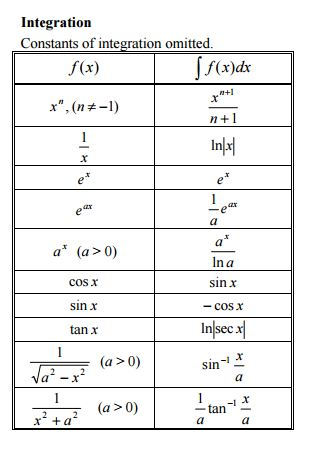
\includegraphics[width=0.55\linewidth]{integrationtabless}
\end{figure}



%Example
%
%\[\int_1^3 9 dx = 9(3-1)=9\cdot 2 = 18.\]
%\[\int_{-2}^6 11 dx = 11(6-(-2))=11\cdot 8 = 88.\]
%\[\int_{2}^{17} 0 dx = 0\cdot(17-2) =0.\]


Addition and Subtraction Rules of Integration
\[\int_a^b (f(x) + g(x)) dx = \int_a^b f(x) dx + \int_a^b g(x) dx.\]

\[\int_a^b (f(x) - g(x)) dx = \int_a^b f(x) dx - \int_a^b g(x) dx.\]


%Example
%
%From above $\int_1^3 9 dx =  18$ and $\int_1^3 2x^2 dx = \frac{52}{3} $so
%
%\[\int_1^3 (2x^2 + 9)dx = \int_1^3 2x^2 dx + \int_1^3 9 dx = \frac{52}{3} + 18 = \frac{106}{3},\]
%\[\int_1^3 (2x^2 - 9)dx = \int_1^3 2x^2 dx - \int_1^3 9 dx = \frac{52}{3} - 18 = -\frac{2}{3}.\]
%
%Example
%
%\[\int_0^2 4x^2 + 14 dx = 4\int_0^2 x^2 dx + \int_0^2 14 dx = 4 \cdot \frac{1}{3}(2^3-0^3) + 2 \cdot 14 = \frac{32}{3} + 28 = \frac{116}{3}.\]

\subsection*{The Power Rule for Integration}
The power rule for derivatives can be reversed to give us a way to handle integrals of powers of x. Since

\[\frac{d}{dx} x^n = n x^{n-1},\]

we can conclude that

\[\int n x^{n-1} \, dx = x^n + C,\]

or, a little more usefully,

\[\int x^n \, dx = \frac{x^{n+1}}{n+1} + C\]
\subsection*{Question 33 : Introduction to Integration}
%=========================== %

\subsubsection*{Part A}
Using appropriate substitutions, evaluate the indefinite integrals:

\begin{multicols}{2}
	\begin{enumerate}[(i)]
		
		\item 
		\[ \int (s - 4)^5 ds \]
		\item 
		\[ \int 
		\frac{3}{(x + 1)^4 }dx\]
		\item 
		\[\int 
		(2y + 3)(y^2 + 3y + 2)^2 dy\]
		
	\end{enumerate}
\end{multicols}

\subsubsection*{Part B}
Using appropriate substitutions, evaluate the indefinite integrals:
\begin{multicols}{2}
	\begin{itemize}
		
		\item[(i)]	
		\[\int 3x^2 (x^3+1)^5 \, dx\]
		
		\item[(ii)]
		\[\int x^4 \sin(x^5) \, dx\]
	\end{itemize}
\end{multicols}
\bigskip
%============================================================================================= %



%========================================================================== %
\subsection*{Question 34 : Integration}
Evaluate the following indefinite integrals using partial fractions:
\begin{multicols}{2}
	\begin{enumerate}[(i)]
		
		\item \[ \int \frac{x}{x^2-9} dx  \]
		
		\item \[ \int \frac{x-2}{x^2 - 4x + 3} dx  \]
		
		\item \[ \int \frac{2x-4}{x^2 - 4x + 8} dx  \]
		
	\end{enumerate}
\end{multicols}


\subsection*{Question 35 : Integration by Parts}
Evaluate the following using integration by parts.

\begin{multicols}{2}
	\begin{enumerate}[(i)]
		\item \[ \int -4\ln\left(x\right)dx\]
		% -4x\ln\left(x\right)+4x+C
		
		\item \[ \int\left(-7x+38\right)\cos\left(x\right)dx\]
		% \left(-7x+38\right)\sin\left(x\right)-7\cos\left(x\right)+C
		
		\item  \[\int_0^\frac{\pi}{2}\left(-6x+45\right)\cos\left(x\right)dx\]
		
		% -3\pi+51
		
		\item \[ \int\left(5x+1\right)\left(x-6\right)^4 dx\]
		
		% \frac{\left(5x+1\right)\left(x-6\right)^5}{5}-\frac{\left(x-6\right)^6}{6}+C
		
		\item \[ \int_{-1}^1 \left(2x+8\right)^3\left(-x+2\right)dx\]
		
		% \frac{9584}{5}
		
		\item \[ \int \sin\left(x\right) e^x\, dx \] 
		% \frac 1 2 e^x\left(\sin\left(x\right) - \cos\left(x\right) \right) +C
	\end{enumerate}
\end{multicols}




%==============================================================================%





%========================================================================== %


\subsection*{Question 36 : Integration by Parts}
\begin{framed}
\noindent	\textbf{Formula:} \\ If u and v are functions of x that have continuous derivatives,
	then
	\[\int udv = uv - \int vdu\]
\end{framed}
\newpage
\subsubsection*{The LIPET rule}
It is considered a rule of thumb to remember the acronym \textbf{LIPET}
when performing integration by parts. This acronym will help you to determine
what to use as $u$. 


\begin{description}
	\item[L]-logarithms, 
	\item[I]-inverse trigonometric functions,
	\item[P]-polynomials (i.e. $x$, $x^2$) , 
	\item[E]-exponentials (i.e. $e^x$, $e^{3x}$), 
	\item[T]-trigonometric functions.
\end{description}

%=================================%
\begin{framed}
	\begin{itemize}
		\item
		$\cosh(x)$ is both the derivative and integral of $\sinh(x)$
		
		\item
		$\sinh(x)$ is both the derivative and integral of $\cosh(x)$
	\end{itemize}
\end{framed}
\subsection*{Question 37 : Integration by Parts}
%Revision Week Exercises
\begin{figure}[h!]
	\centering
	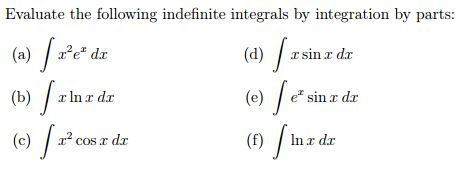
\includegraphics[width=0.7\linewidth]{Question26integrationbyparts}
\end{figure}
\subsection*{Question 38 : Integration (Video)}
% - http://en.wikibooks.org/wiki/Calculus/Integration/Exercises
Evaluate the following:
\begin{multicols}{2}
	\begin{itemize}
		
		\item[(i)] \[\int x^2-(2x)^{2}\, dx\]
		\item[(ii)] \[\int 8x^3\, dx\]
		\item[(iii)]\[ \int (4x^2+11x^3)\, dx\]
		\item[(iv)] \[\int (31x^{32}+4x^3-9x^4) \,dx\]
		\item[(v)] \[\int 5x^{-2}\, dx\]
	\end{itemize}
\end{multicols}







%===============================================================================%


\subsection*{Question 39 : Definite Integrals (Video)}
Evaluate the following definite integrals 


\begin{multicols}{2}
	\begin{enumerate}[(i)]
		\item \[ \int^{2}_{1} (x^2-1) dx \]
		
		%	\item  \[ \int^{2}_{0} x^2+1 dx \]
		
		\item \[ \int^{\frac{\pi}{2}}_{0} \cos x dx \]
		
		\item \[ \int^{\pi}_{0} \cos x dx \]
		
		\item \[ \int^{2}_{1} (y^2 - y^{-2}) dy \]
		
		% - \item \[ \int^{2}_{1} y^2+y{-2} dx \]
		
		\item \[ \int^{1}_{-3} (6x^2 -5x + 2)dx \]
		
		% - \item \[ \int^{1}_{-3} \int 6x^2 -5x +2 dx \]
		
		
		
		\item \[ \int^0_4 \sqrt{t}(t-2) dt \]
		
		% - \item \[ \int^{0}_{4} \sqrt{t}(t-2) dt \]
		
		
		% - http://tutorial.math.lamar.edu/Classes/CalcI/ComputingDefiniteIntegrals.aspx#Int_CompDef_Ex3a
		
		% -	\item \[ \int^{2}_{1} \frac{2w^5 - w + 3}{w^2} dw \]
		
		% - \item \[ \int^{2}_{1} dR \]
	\end{enumerate}
\end{multicols}
%-------------------------------------------------%

\begin{framed}
	\textbf{Hint:} 
	\[ \int \sqrt{t}(t-2) dt \]
	
	\[ \sqrt{t}(t-2) = t^{1/2} \times (t - 2) = t^{3/2} - 2t^{1/2}\]
	
\end{framed}
%--------------------------------------------------%


% \[ x^2 - 4x + 3 = (x-1)(x-3) \]

% \[ \int \frac{}{} dx \]

%============================================================================================= %
\subsection*{Question 40 : Definite Integrals (Video)}
\begin{figure}[h!]
	\centering
	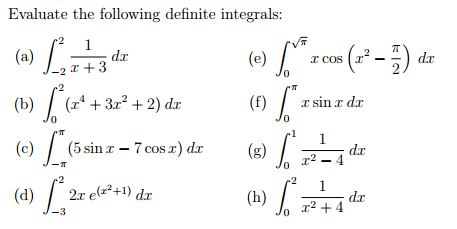
\includegraphics[width=0.8\linewidth]{Question25}
\end{figure}
\newpage
%============================================================================================= %
%=============================================================================================================== %
% Appilcations of Integration


\subsection*{Question 41 : Definite Integrals}
\begin{framed}
	{\large
		\noindent \textbf{Exercise}: Evaluate the following definite integral
		\[ \int^{3}_{1} \frac{x}{3}  dx \]
		\textbf{Solution}
		\[ \int^{3}_{1} \frac{x}{3}  dx  = \left[\frac{x^4}{4}\right]^{3}_{1}= \frac{81}{4} - \frac{1}{4} = 20\]
	}
\end{framed}
\newpage
%=========================== %
\begin{framed}
	{\large
		\noindent \textbf{Exercise}: Evaluate the following definite integral
		
		\[ \int^3_1 \frac{x^2 - 4x + 3}{x-3}  dx \] 
		
		\noindent	Factorize the numerator $x^2 - 4x + 3 = (x-1)(x-3)$
		
		
		Treat it as an indefinite integral for time being.			
		\[ \int \frac{x^2 - 4x + 3}{x-3}  dx = \int \frac{(x-1)(x-3)}{x-3}  dx  = \int (x-1) dx = \frac{x^2}{2} -x +c\] 
		
		\[ \left[ \frac{x^2}{2} -x\right]^{3}_{1} = (4.5-3)-(0.5-1) = 2\]
	}
\end{framed}


\subsection*{Question 42 : Integration by Parts (Exam Standard)}	
the following questions are from previous past papers. Please be advised of the notes below.
\begin{enumerate}[(i)]
	\item (2005) Use integration by parts to find $\displaystyle{\int xe^xdx}$ 
	
	\item (2006) Use integration by parts to find $\displaystyle{\int x ln(x) dx}$ 
	
	\item (2007) Use integration by parts to find $\displaystyle{\int x sinh(x) dx}$ 
	
	\item (2008) Use integration by parts to find $\displaystyle{\int x cos(x) dx}$ 
	
	\item (2009) Use integration by parts to find $\displaystyle{\int x cosh(x) dx}$ 
	
	\item (2010) Use integration by parts to find $\displaystyle{\int xe^xdx}$ 
\end{enumerate}

% - http://www.math.uri.edu/~adamgilbert/Documents/Calculus/Notes/MTH142/IntegrationByParts.pdf
\newpage
\begin{framed}
	\noindent \textbf{Important:	}
	\begin{itemize}
		\item You should expect to see hyperbolic functions (i.e. $\cosh(x)$ and $\sinh(x)$)  in the end of semester exam. 
		\item However you should expect to see terms like $ x^2$, $e^{2x}$ and $ \ln(x)$, as well as what was in previous exams.
		\item \textbf{VERY Important:} Make sure you know how to integrate and differentiate expressions of the form $e^{ax}$, $\cos(ax)$, $\cosh(ax)$ , $\sin(ax)$ and $\sinh(ax)$. 
	\end{itemize}
\end{framed}

%================================================= %
\subsection*{Question 43 : Definite Integrals}
Evaluate the following definite integrals 

\begin{enumerate}[(i)]
	
	\item 
	% - Lecture Notes Definite Integral
	% Examples 5 to 7
	Find the area between $f(x) = x^2 + 4x $ and the $x-$axis between 
	$x=-4$   and $ x=3$.
	
	\item Calculate the following:
	\[ \int^{1}_{0} \frac{4x^3}{x^4+1} dx \]
	
	
	\item Evaluate 
	
	\[ \int^{\frac{\pi}{2}}_{0} \cos^4(x) \sin(x) dx \]
\end{enumerate}
\end{document}
